\documentclass[12pt,a4paper]{article}
\usepackage{amsmath,amscd,amsbsy,amssymb,latexsym,url,bm,amsthm}
\usepackage{epsfig,graphicx,subfigure}
\usepackage{enumitem,balance}
\usepackage{wrapfig}
\usepackage{mathrsfs,euscript}
\usepackage[usenames]{xcolor}
\usepackage{hyperref}
\usepackage{float}
\usepackage[vlined,ruled,linesnumbered]{algorithm2e}
\hypersetup{colorlinks=true,linkcolor=black}

\newtheorem{theorem}{Theorem}
\newtheorem{lemma}[theorem]{Lemma}
\newtheorem{proposition}[theorem]{Proposition}
\newtheorem{corollary}[theorem]{Corollary}
\newtheorem{exercise}{Exercise}
\newtheorem*{solution}{Solution}
\newtheorem{definition}{Definition}
\theoremstyle{definition}

\renewcommand{\thefootnote}{\fnsymbol{footnote}}

\newcommand{\postscript}[2]
 {\setlength{\epsfxsize}{#2\hsize}
  \centerline{\epsfbox{#1}}}

\renewcommand{\baselinestretch}{1.0}

\setlength{\oddsidemargin}{-0.365in}
\setlength{\evensidemargin}{-0.365in}
\setlength{\topmargin}{-0.3in}
\setlength{\headheight}{0in}
\setlength{\headsep}{0in}
\setlength{\textheight}{10.1in}
\setlength{\textwidth}{7in}
\makeatletter \renewenvironment{proof}[1][Proof] {\par\pushQED{\qed}\normalfont\topsep6\p@\@plus6\p@\relax\trivlist\item[\hskip\labelsep\bfseries#1\@addpunct{.}]\ignorespaces}{\popQED\endtrivlist\@endpefalse} \makeatother
\makeatletter
\renewenvironment{solution}[1][Solution] {\par\pushQED{\qed}\normalfont\topsep6\p@\@plus6\p@\relax\trivlist\item[\hskip\labelsep\bfseries#1\@addpunct{.}]\ignorespaces}{\popQED\endtrivlist\@endpefalse} \makeatother

\begin{document}
\noindent

%========================================================================
\noindent\framebox[\linewidth]{\shortstack[c]{
\Large{\textbf{Lab02-Divide and Conquer}}\vspace{1mm}\\
CS214-Algorithm and Complexity, Xiaofeng Gao, Spring 2021.}}
\begin{center}
\footnotesize{\color{red}$*$ If there is any problem, please contact TA Haolin Zhou. }

\footnotesize{\color{blue}$*$ Name:BeichenYu  \quad Student ID:519030910245 \quad Email: polarisybc@sjtu.edu.cn}
\end{center}

\begin{enumerate}
\item
    \textit{Recurrence examples.} Give asymptotic upper and lower bounds for $T(n)$ in each of the following recurrences. Assume that $T(n)$ is constant for sufficiently small $n$. Make your bounds as tight as possible.
\begin{enumerate}
	\item $T(n)=4 T(n / 3)+n \log n$
	\item $T(n)=4 T(n / 2)+n^{2} \sqrt{n}$
	\item $T(n)=T(n-1)+n$	
	\item $T(n)=2T(\lfloor \sqrt n\rfloor)+\log n$
\end{enumerate}

\begin{solution}
    First we have the master theorem:
    \begin{align*}
    T(n)&=aT(\lceil\dfrac{n}{b}\rceil)+O(n^d)\\
    &=\left\{  
\begin{aligned}
&O(n^d)&,b^d>a\\
&O(n^d\log n)&,b^d=a\\
&O(n^{\log_{b} a})&,b^d<a
\end{aligned}
\right.  
    \end{align*}
	\begin{enumerate}
	\item $T(n)=4 T(n / 3)+n \log n$
	
	As $T(n)\geqslant0$ is always right, we know that $T(n) = \Omega(n\log n)$.
	
	Next we consider scaling from another direction. We know that $n\log n = O(n^{1+\epsilon})$, in which $\epsilon)$ is a really small number which is close to zero. So we can rewrite the recurrence into $T(n)=4 T(n / 3)+O(n^{1+\epsilon})$. Then we can use the master theorem. Because $a=4$, $b=3$ and $d=1+\epsilon$, $b^d <a$, we know that $T(n) = O(n^{\log_3 4})$.
	
	So we conclude that $T(n)= \Omega(n\log n)$ and $T(n) = O(n^{\log_3 4})$.\\
	
	\item $T(n)=4 T(n / 2)+n^{2} \sqrt{n}$
	
	This time we can use the master theorem directly. $a=4$, $b=2$, and $d= \frac{5}{3}$, so $b^d>a$. According to the master theorem, we have $T(n) = O(n^{\frac{5}{2}})$. At the same time, we can make sure that $T(n) = \Omega(n^{\frac{5}{2}})$ as  $T(n)\geqslant0$, so $T(n) = \Theta(n^{\frac{5}{2}})$.\\
	
	\item $T(n)=T(n-1)+n$	
	
	We can use our knowledge of the Arithmetic sequence to solve it. Because that $T(n)$ is constant for sufficiently small $n$, we assume $T(1) = 1$. And $T(n) - T(n-1) = n$. So $T(n) = 1+2+\cdots+n=\frac{1}{2}n(n+1)$, which means $T(n) =\Theta(n^2)$.\\
	
	\item $T(n)=2T(\lfloor \sqrt n\rfloor)+\log n$
	
	First let us do some calculations:
	\begin{align*}
	T(n)&\approx 2T(n^{\frac{1}{2}})+\log n\\
	&\approx2(2T(n^{\frac{1}{4}})+\log n^{\frac{1}{2}})+\log n\\
	&=4T(n^{\frac{1}{4}})+2 \log n\\
	&\approx 8T(n^{\frac{1}{8}})+2\log n\\
	&\approx \cdots\\
	&\approx 2^kT(n^{\frac{1}{2^k}})+k\log n
	\end{align*}
	Now we have to confirm the value of $k$. 
	
	When will $n^{\frac{1}{2^k}}$ be a constant? We let the expression be equal to 2:
	\begin{align*}
	n^{\frac{1}{2^k}} &= 2\\
	2^{2^{k}} &= n\\
	2^k &= \log n\\
	k &= \log \log n
	\end{align*}
	So when $T(n^{\frac{1}{2^k}}) = 1$, we have $k = \log \log n$. As $2^k = 2^{\log \log n} = \log n$, we know that $T(n) = \Theta(\log n \cdot \log \log n)$.
    \end{enumerate}
\end{solution}
\item
\textit{Divide-and-conquer.} Given an integer array $A[1..n]$ and two integers $lower \le upper$, design an algorithm using \textbf{divide-and-conquer} method to count the number of ranges $(i,j)$ ($1 \leq i \leq j \leq n$) satisfying
$$
    lower \leq \sum_{k=i}^{j}{A[k]} \leq upper.
$$
\textbf{Example:}

Given $A = [1,-1,2]$, $lower = 1$, $upper = 2$, return 4.

The resulting four ranges are $(1,1)$, $(3,3)$, $(2,3)$ and $(1,3)$.

\begin{enumerate}
\item
Complete the implementation in the provided C/C++ source code.
\item
Write a recurrence for the running time of the algorithm and solve it by recurrence tree.
\item
Can we use the Master Theorem to solve the recurrence above? Please explain your answer.
\end{enumerate}
\begin{solution}
\begin{enumerate}
\item I have finish the \textit{Code-Range.cpp}, and my source code is included in the zip.

\item The time complexity of the binary searching in the loop and the sorting are both $O(nlogn)$. Each time the question is divided into two parts, and doing the merging twice. So we can write down the recurrence:
$$T(n) = 2T(\frac{n}{2})+O(n\log n)$$

And we can draw the recurrence tree as well.
\begin{figure}[H]
    \centering
    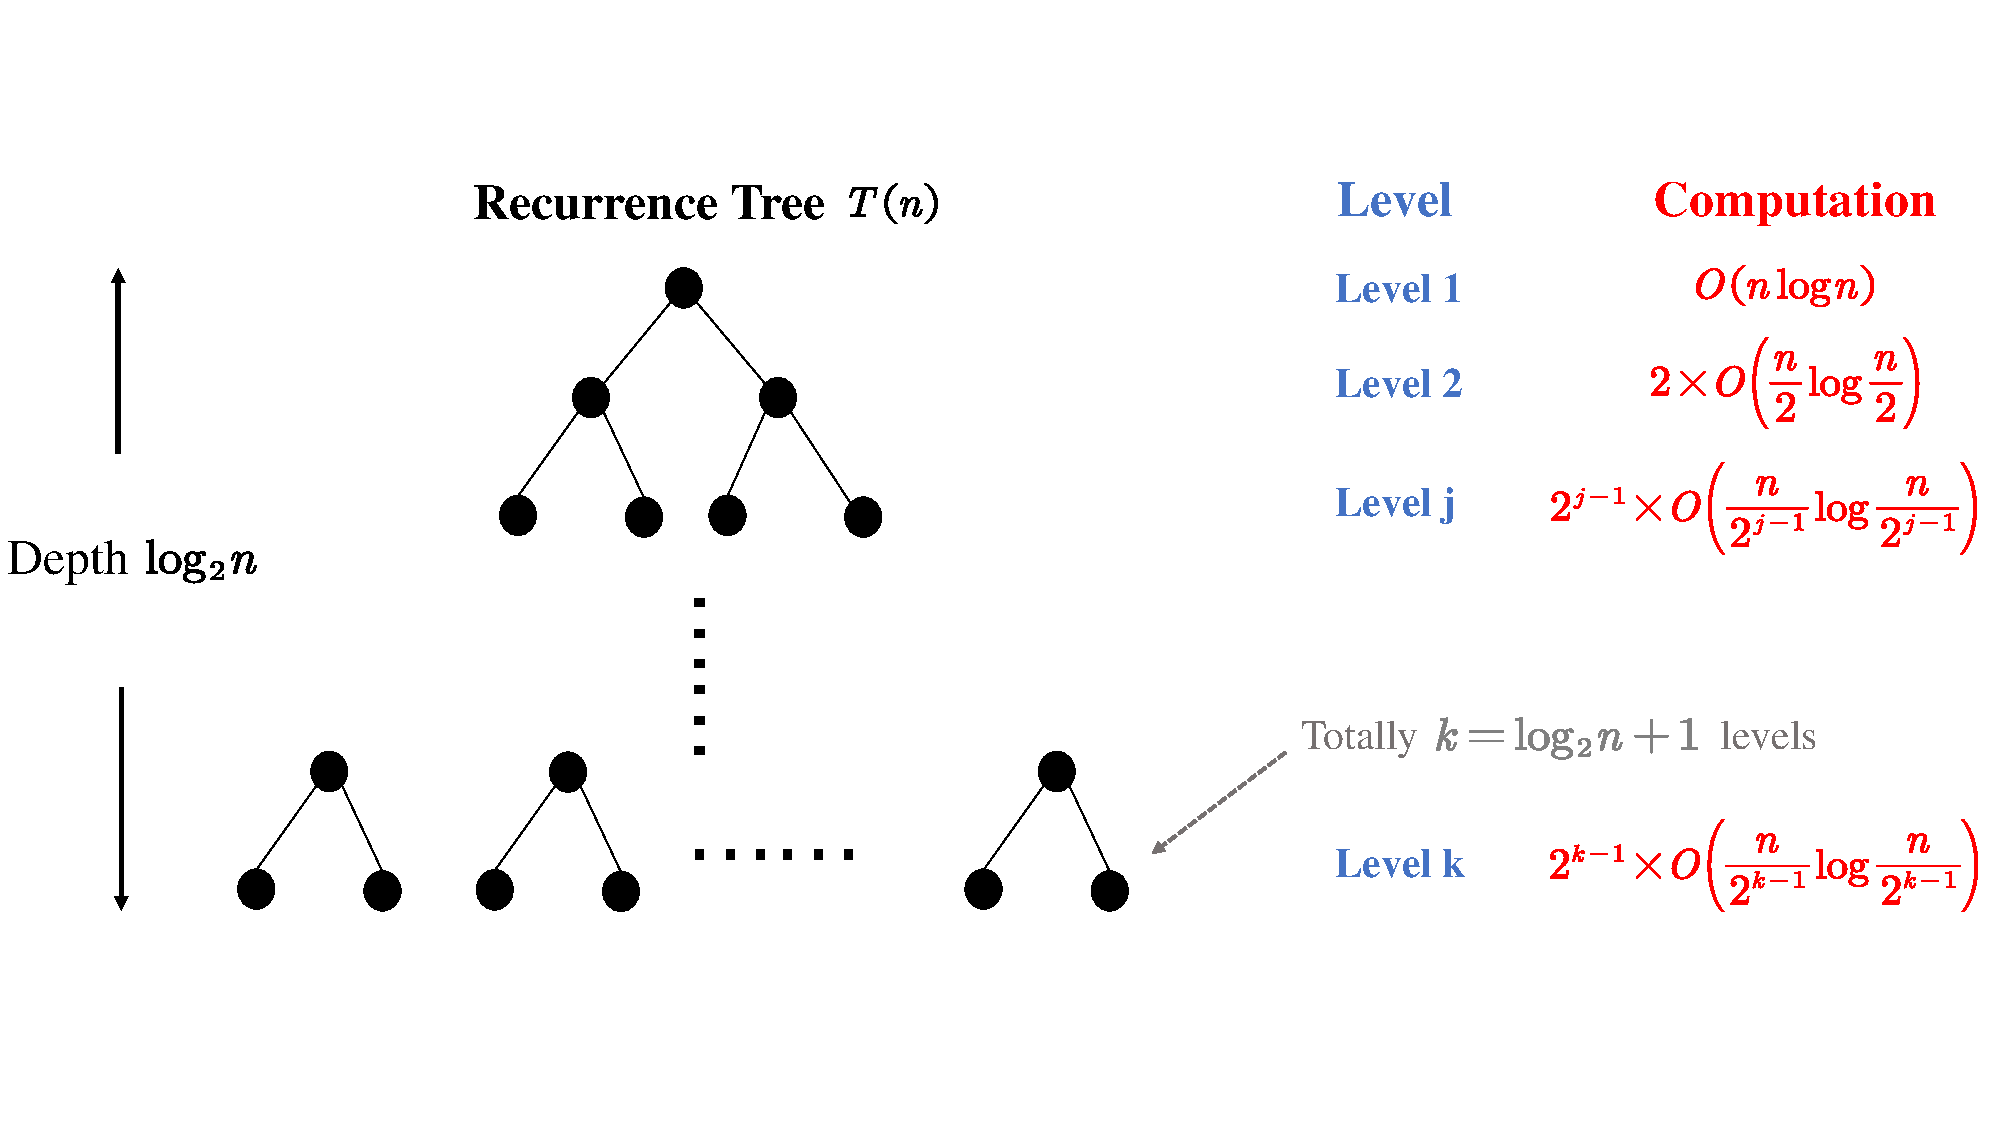
\includegraphics[width=0.6\textwidth]{Fig-RecurrenceTree.pdf}
    \caption{The recurrence tree}\label{Fig-RecurrenceTree}
\end{figure}

So we have: 
\begin{align*}
T(n) &= \sum_{j=1}^{1+\log_2 n}2^{j-1}\times O(\frac{n}{2^{j-1}}\log \frac{n}{2^{j-1}}) = \sum_{j=0}^{\log_2 n}  O(n\log\frac{n}{2^j})\\
&=  \sum_{j=0}^{\log_2 n} O(n\log n - jn) = n\log n(\log n +1) - n\frac{\log n(\log n +1)}{2} = \Theta(n\log^2 n)
\end{align*}

\item 
We can not use the Master Theorem to solve this problem. We know $n\log n = O(n^{1+\epsilon})$, in which $\epsilon$ is a small number which is close to zero. When comparing $b^d$ with $a$, we will meet some problem. We know that $b = a = 2$, but it is wrong to say either $2^{1+\epsilon} > 2$ or $2^{1+\epsilon} = 2$. In fact the two expression cannot compare like this. That is to say, the Master Theorem has no effect in solving this problem.
 
\end{enumerate}
\end{solution}
\item
\textit{Transposition Sorting Network.} A comparison network is a \textbf{transposition network}  if each comparator connects adjacent lines, as in the network in Fig.~\ref{Fig-Transposition}.

\begin{figure}[htbp]
    \centering
    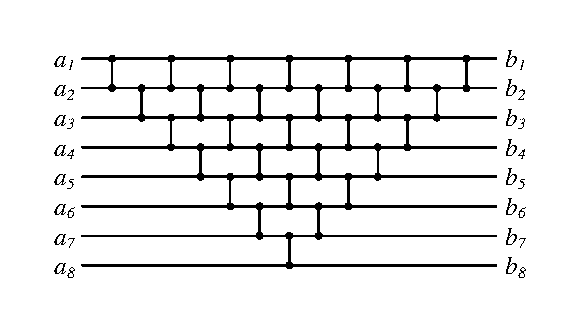
\includegraphics[width=0.4\textwidth]{Fig-Transposition.pdf}
    \caption{A Transposition Network Example}\label{Fig-Transposition}
\end{figure}

\begin{enumerate}
\item Prove that a transposition network with $n$ inputs is a sorting network if and only if it sorts the sequence $\langle n, n-1, \cdots, 1 \rangle$. {\color{blue}(Hint: Use an induction argument analogous to the \emph{Domain Conversion Lemma}.)}
\item {\color{red}{(Optional Sub-question with Bonus)}} Given any $n \in \mathbb{N}$, write a program using Tkinter in Python to draw a figure similar to Fig.~\ref{Fig-Transposition} with $n$ input wires.
\end{enumerate}

\begin{solution}

\begin{enumerate}
\item 

(To solve the problem, I referred to the solution of the 27th section of CLRS book, 2nd edition.)\\

We use $D_0$ to on behalf of the sequence $\langle n, n-1, \cdots, 1 \rangle$, and $X_0$ to on behalf of any possible input sequence $\langle x_1, x_2, \cdots, x_n \rangle$. We number the comparator in order from left to right. Each time when the input sequence passing by a comparator, the sequence may take a change, and we sign the sequence just passed by the comparator $k$ as $D_k$ or $X_k$. And we sign the $i$-th number in the sequence, which means it is on the $i$-th line at that time, as $D_k(i)$ or $X_k(i)$.\\
 
To solve the problem, first we can try to prove the proposition below:\\

For $\forall k$, if $\forall i<j$ and $D_k(i)<D_k(j)$, then $X_k(i)<X_k(j)$.\\

We use induction to prove it.\\

First, when $k=0$, $\forall i<j$, $D_k(i) = n -i > D_k(j) = n-j$, so $D_k(i)<D_k(j)$ will never happen. So the proposition is true. We assume that $i<j$ and $D_k(i)<D_k(j)$, next we will prove that $X_k(i)<X_k(j)$.\\

Second, we assume that when the sequence just passed by the comparator $k-1$, the proposition is true. Next we have to prove that when the sequence just passed by the comparator $k$, the proposition is true. Let us discuss it by cases.\\

Case 1: Line $i$ and line $j$ are just the upper and lower sides of the $k$-th comparator. With the effect of the comparator, $X_k(i)<X_k(j)$ is obviously.\\

Case 2: Both of line $i$ and line $j$ are not the upper and lower sides of the $k$-th comparator. So both of
them do not change value during this process. So $D_k(i)<D_k(j)$ means $D_{k-1}(i)<D_{k-1}(j)$, and by the inductive assumption $X_{k-1}(i)<X_{k-1}(j)$, then $X_{k}(i)<X_{k}(j)$ is true.\\

Case 3: Line $i$ is the upper side of the $k$-th comparator, and $j>i+1$. That is to say, line $j$ is under the lower side of the $k$-th comparator. By the inductive assumption $X_{k-1}(i)<X_{k-1}(j)$, so after passing the comparator, if the exchange happened, $X_k(j) = X_{k-1}(j) > X_{k-1}(i) = X_k(i+1) > X_k(i)$; if the exchange did not happen, $X_k(j) = X_{k-1}(j) > X_{k-1}(i) = X_k(i)$. So $X_{k}(i)<X_{k}(j)$ is true.\\

Case 4: Line $i$ is the lower side of the $k$-th comparator, and $j>i+1$. That is to say, line $j$ is under the lower side of the $k$-th comparator. After passing the comparator, if the exchange happened, $D_k(i) = D_{k-1}(i-1)$, so $D_{k-1}(i-1) = D_k(i) < D_k(j) = D_{k-1}(j)$, as $i-1 <j$, by the inductive assumption we have $X_{k-1}(i-1) < X_{k-1}(j)$, the $X_{k}(i)<X_{k}(j)$; if the exchange did not happen, $X_k(j) = X_{k-1}(j) > X_{k-1}(i) = X_k(i)$. So $X_{k}(i)<X_{k}(j)$ is true.\\

Case 5: Line $j$ is the lower side of the $k$-th comparator, and $i<j-1$. That is to say, line $i$ is above the upper side of the $k$-th comparator. The same as Case 3.\\

Case 6: Line $j$ is the upper side of the $k$-th comparator, and $i<j-1$. That is to say, line $i$ is above the upper side of the $k$-th comparator. The same as Case 4.\\

The 6 cases are all the cases, so the proposition is proved.\\

In particular, if $k$ is the number of the comparators int the transposition network, then $D_k$ and $X_k$ are the final output. Because $\forall i<j$ we have $D_k(i) = i < D_k(j) = j$, according to the proposition we proved above, $X_k(i)  < X_k(j)$. That means the transposition network is a sorting network. 

\item

The source code ``drawing.py" is in the .zip file.
\begin{figure}[H]
\centering
\begin{minipage}[t]{0.48\textwidth}
\centering
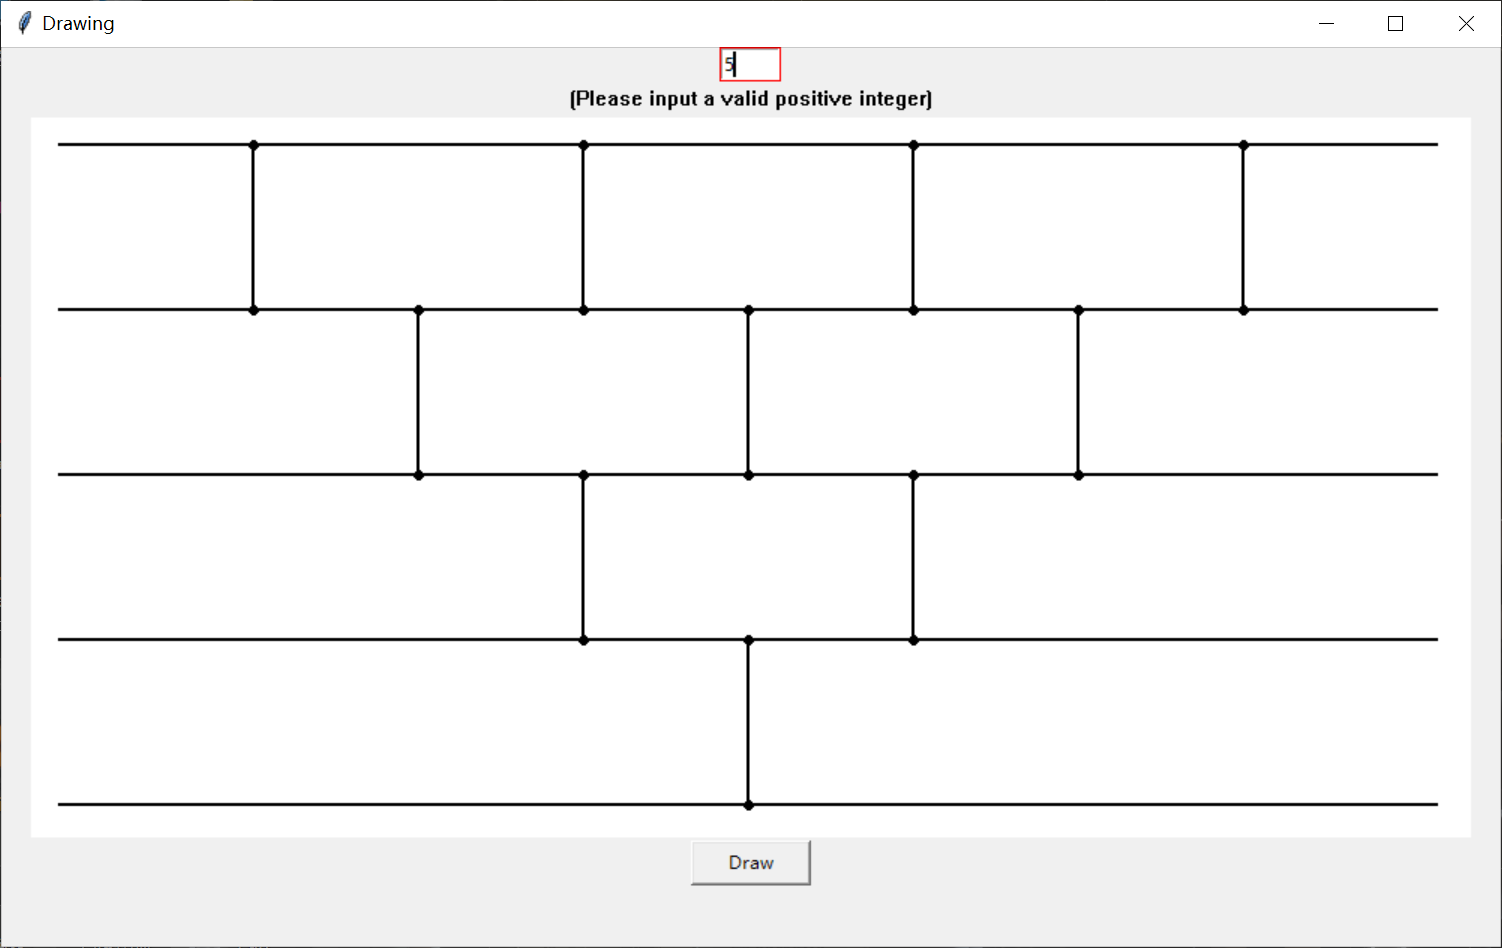
\includegraphics[width=7.5cm]{n=5.png}
\caption{n = 5}
\end{minipage}
\begin{minipage}[t]{0.48\textwidth}
\centering
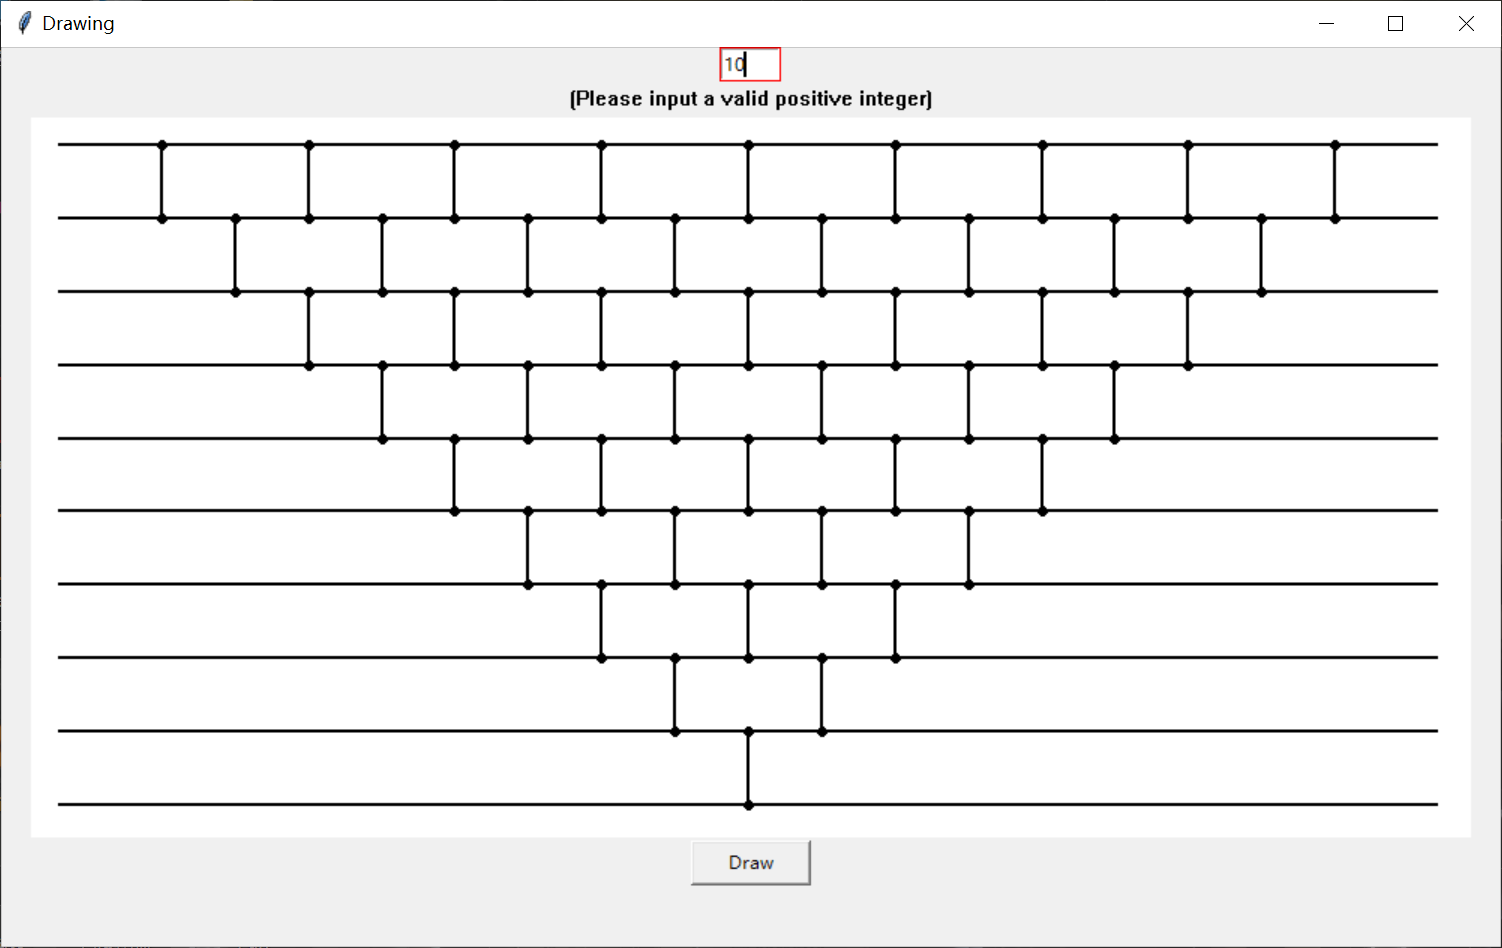
\includegraphics[width=7.5cm]{n=10.png}
\caption{n = 10}
\end{minipage}
\end{figure}

\begin{figure}[H]
\centering
\begin{minipage}[t]{0.48\textwidth}
\centering
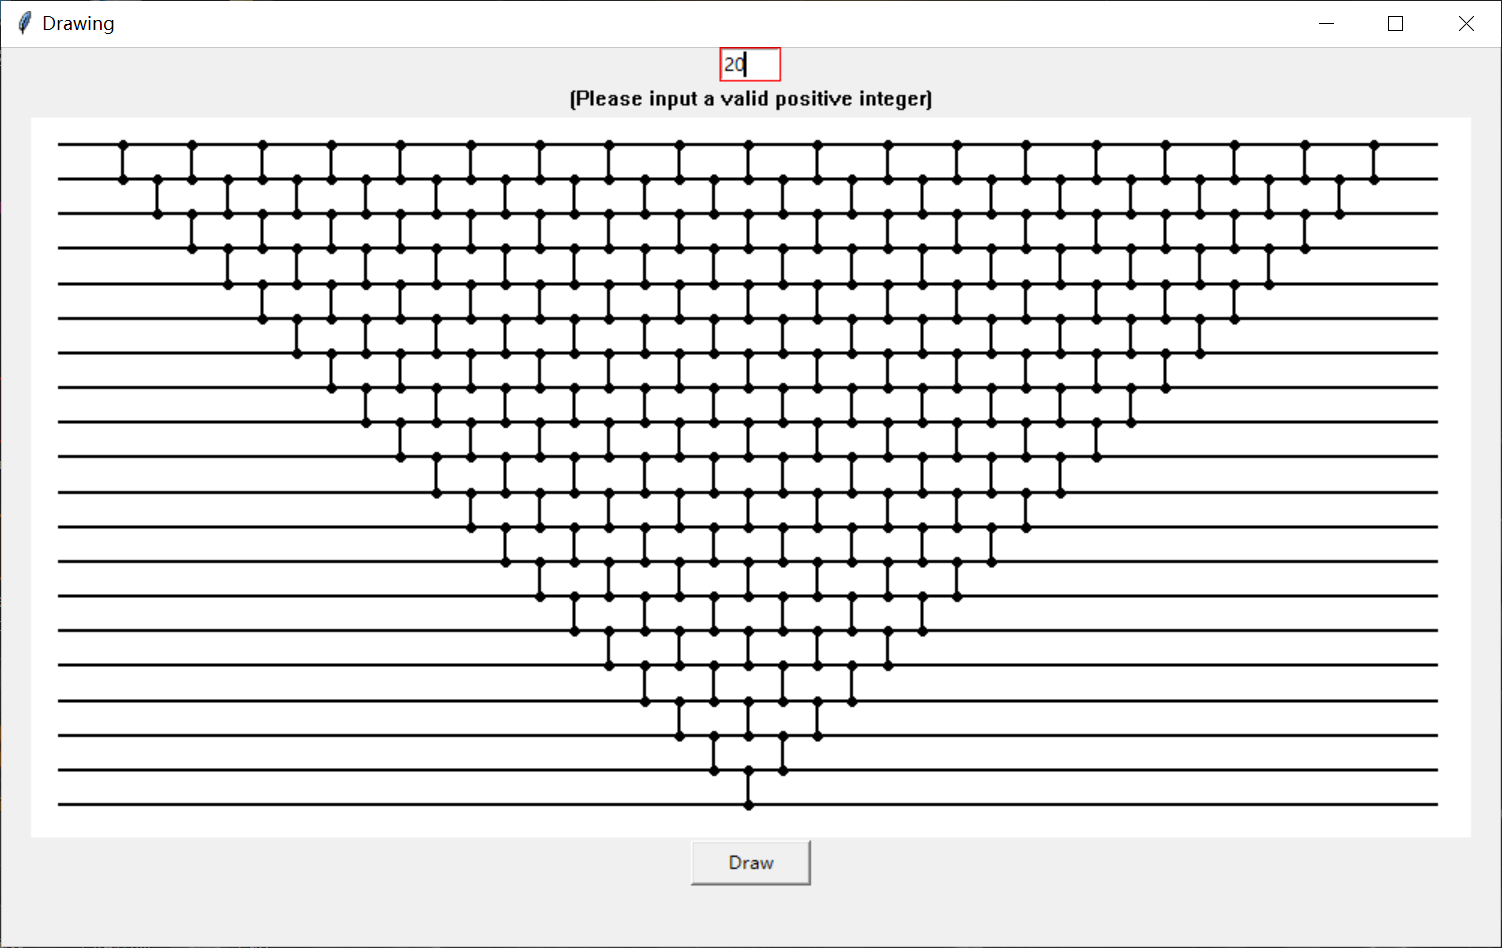
\includegraphics[width=7.5cm]{n=20.png}
\caption{n = 20}
\end{minipage}
\begin{minipage}[t]{0.48\textwidth}
\centering
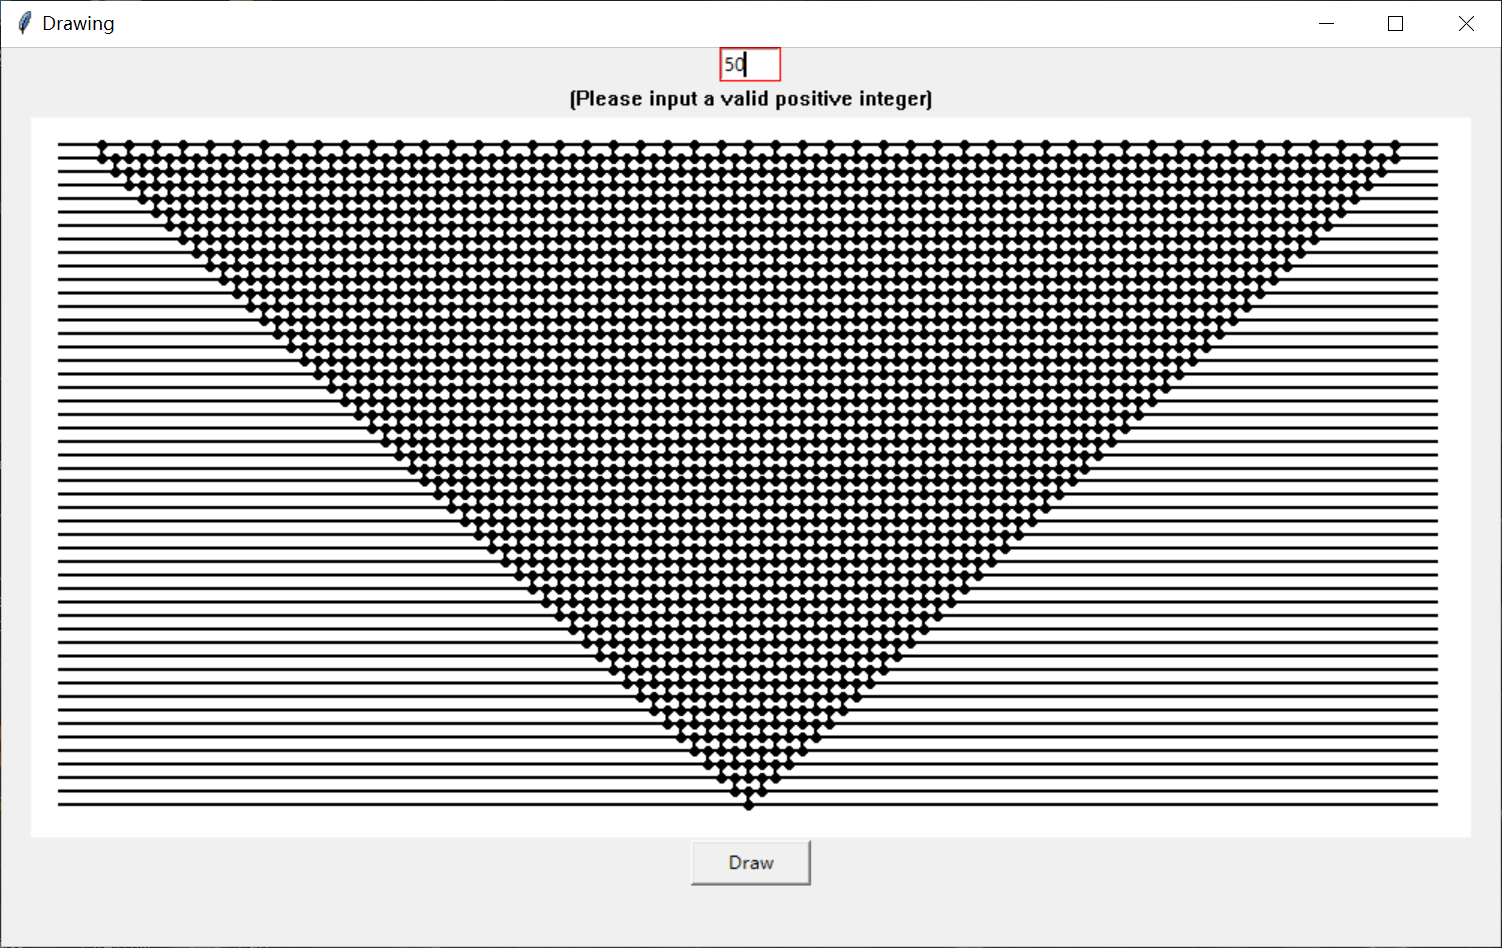
\includegraphics[width=7.5cm]{n=50.png}
\caption{n = 50}
\end{minipage}
\end{figure}


\end{enumerate}


\end{solution}
\end{enumerate}

%========================================================================
\end{document}
